% Based on: anchor/ paper draft.

\chapter{Behavioral Anchor Conditioning for Constrained Trajectory Diffusion}
\label{ch:seeding}

\cref{ch:payload} showed that conditioning a trajectory diffusion model on a single governing property---payload mass---is enough to make generated motions respect the dynamic constraints that property induces.
This chapter asks how far that principle extends when no single scalar captures the relevant constraints.
Instead of conditioning on a hand-chosen property, it represents an environment by its \emph{behavioral} response to a set of diagnostic motion probes, yielding a compact, constraint-agnostic conditioning signal.
The goal shifts accordingly: rather than producing directly executable trajectories, the model amortizes constraint reasoning into near-feasible \emph{seeds} that make downstream trajectory optimization converge faster and more reliably.

% ── 1. Introduction ──────────────────────────────────────────────────────────

\section{Introduction}\label{sec:introduction}

Diffusion-based policies can learn expressive motion priors from demonstrations and can enable generalization across tasks.
In planning settings, generation must be environment-conditioned: the same start and goal can require very different trajectories depending on the constraints imposed by the scene or task.
This makes the conditioning representation central to the success of the model, since the diffusion model can only generate appropriate trajectories if its condition captures the environment differences that matter for motion.

Constraint information, including kinematic and dynamic constraints derived from scene, robot embodiment, and task, enter the trajectory denoising model through a learned observation embedding via FiLM, concatenation, or cross-attention.
A common approach is to condition on high-dimensional perceptual inputs, such as RGB images, depth maps, point clouds, occupancy grids, or learned visual embeddings.
These representations are intuitively appealing because they preserve scene information, moving from appearance-level information in RGB toward more explicit geometric information in depth or point clouds.

However, perceptual richness does not guarantee behavioral usefulness: a representation may preserve visual or geometric variation that is irrelevant to planning, while discarding subtle constraint-relevant variation.
% The key abstraction problem is therefore not ``which sensor modality is most detailed?'' but ``which representation preserves the distinctions that change feasible motion?''
For trajectory diffusion, two environments should be considered equivalent if they induce the same or similar feasible trajectory distribution, even if they look different perceptually.
Conversely, two perceptually similar environments should be represented differently if they force different trajectory behavior, for example because a small geometric or dynamic change makes one class of motions infeasible.
This motivates behavioral equivalence (not perceptual similarity) as the right level of abstraction: the conditioning variable should collapse perceptual variance that does not affect motion, while preserving constraint-induced differences that do.
This notion is constraint-agnostic: the relevant constraints may be kinematic, geometric, dynamic, torque-based, contact-based, safety-related, or task-specific; the representation only needs to encode how those constraints affect feasible motion.
Figure~\ref{fig:anchor_selection} illustrates the anchor-selection process and the construction of binary environment signatures from diagnostic feasibility probes.

% The method presented in this paper approximates behavioral equivalence through diagnostic trajectory snippets, where each snippet acts as a probe applied to an environment under the chosen constraint model.
% Each probe produces a binary constraint-response bit, indicating whether that snippet satisfies the environment's constraints or violates them, regardless of the underlying reason for failure.
% A set of selected snippets therefore assigns each environment a binary feasibility signature, or behavioral barcode, whose coordinates correspond to fixed diagnostic probes evaluated under the relevant constraint model.
% The entropy-style greedy selection algorithm identifies informative anchors by choosing snippets that make these signatures maximally distinguishable, yielding a compact, task-aligned conditioning representation that abstracts away raw perception and preserves the constraint-induced distinctions needed for trajectory diffusion.

This chapter introduces behavioral anchor conditioning, a method for constructing compact environment codes for trajectory diffusion from binary feasibility responses to diagnostic trajectory snippets. Each snippet acts as a fixed motion probe, and each environment is represented by the vector of feasibility outcomes produced by evaluating those probes under the environment's constraint model. The resulting signature is not intended to reconstruct the scene. Instead, it is designed to preserve distinctions that affect feasible motion. In the empirical evaluation, this chapter studies the collision-avoidance setting, where the feasibility oracle is a geometric collision checker. The broader formulation is compatible with other binary constraint oracles, but the quantitative results in this chapter focus on collision-aware trajectory generation.


% ── 2. Related Work ───────────────────────────────────────────────────────────

\begin{figure*}
  \centering
    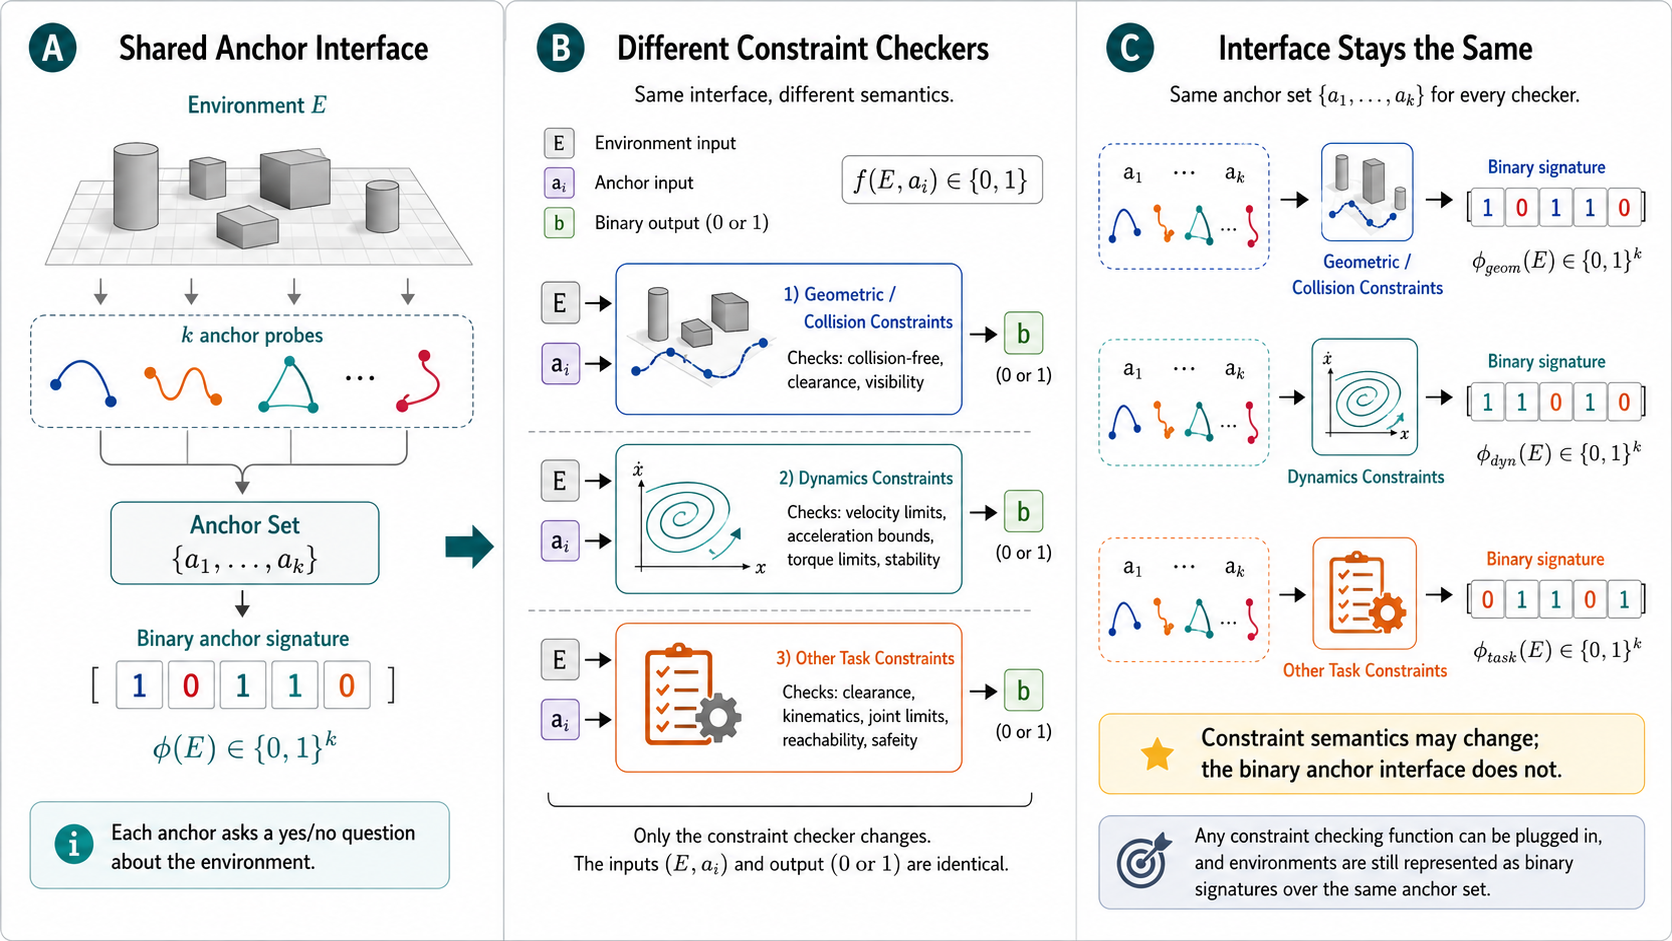
\includegraphics[width=\textwidth]{../anchor/figs/explanatory.png}
  \caption[Diagnostic anchor selection via binary feasibility oracle.]{Diagnostic anchor selection. Candidate trajectory snippets are evaluated across environments using a binary feasibility oracle. Snippets that produce the same response in every environment provide little information, while snippets that split currently indistinguishable environments refine the behavioral signature. The selected anchors define a compact binary code for each environment, where environments with identical signatures are treated as equivalent by the downstream trajectory diffusion model.}\label{fig:anchor_selection}
\end{figure*}

\section{Related Work}\label{sec:related-work}

\textbf{Diffusion models for robot trajectories.}
Diffusion models have recently become a powerful class of generative priors for robot decision making and trajectory generation. Diffuser formulates planning as iterative denoising over trajectories, showing that a diffusion model can represent flexible, multimodal behavior in sequential decision problems~\cite{janner2022diffuser}. Diffusion Policy extends this idea to visuomotor control by learning a conditional denoising process over action sequences and executing the generated actions in a receding-horizon manner~\cite{chi2025diffusionpolicy}. Subsequent work has improved the structure of the generated trajectories and the observation conditions used to guide denoising. ChainedDiffuser combines keypose prediction with local trajectory diffusion for manipulation~\cite{xian2023chaineddiffuser}, while 3D Diffuser Actor denoises end-effector pose trajectories conditioned on tokenized 3D scene features, language, and proprioception~\cite{ke2025threediffuseractor}. DP3 similarly argues that compact point-cloud observations provide a strong interface between 3D perception and diffusion-policy learning~\cite{ze20243d}. In motion planning, Motion Planning Diffusion learns trajectory priors that can seed optimization-based planners~\cite{carvalho2023motionplanningdiffusion}. These works demonstrate that diffusion models can represent expressive trajectory distributions, but they generally assume that the conditioning representation already exposes the environment differences that matter for feasible motion.

\textbf{Environment representations for learning-based planning.}
A central question in learning-based planning is how to encode the scene so that a policy or planner can generalize across environments. Early neural motion-planning work encoded workspaces from point clouds or learned obstacle features, showing that learned representations can accelerate collision-free planning in unseen scenes~\cite{strudel2021obstacle}. More recent diffusion-based planners and manipulation policies have moved toward structured 3D, object-centric, and affordance-based conditions. PRESTO represents the environment using sparse key configurations that approximate configuration-space obstacles for diffusion-based trajectory seeding~\cite{seo2024presto}. Lan-o3dp conditions a diffusion policy on language-selected, task-relevant object point clouds and uses denoising-time cost guidance for collision avoidance~\cite{li2024lano3dp}. SPOT represents manipulation tasks through object-centric SE(3) pose trajectories and uses these trajectories to condition a diffusion policy~\cite{hsu2025spot}. AffordDP further conditions diffusion policies on transferable affordances, represented through 3D contact points and post-contact trajectories, to improve generalization to novel object categories~\cite{wu2025afforddp}. These approaches reduce dependence on raw appearance by introducing geometric, object-level, or affordance-level structure. However, their abstractions are still primarily organized around what is perceived in the scene, rather than around which motions the scene permits or forbids.

\textbf{Behaviorally aligned abstraction.}
Our work is closest in spirit to representation-learning approaches that define abstraction by behavioral relevance rather than perceptual similarity. DeepMDP learns latent models whose representations preserve reward and transition structure~\cite{gelada2019deepmdp}, and deep bisimulation methods learn visual-control representations that discard task-irrelevant variation while preserving control-relevant dynamics~\cite{zhang2020invariant}. Language-guided state abstraction similarly seeks task-aligned state descriptions that suppress irrelevant observation dimensions for imitation learning~\cite{peng2024languageguided}. We adopt the same high-level principle, but instantiate it for environment-conditioned trajectory diffusion. Instead of asking a learned visual embedding to infer which perceptual differences affect planning, we define an environment through its binary responses to a fixed set of diagnostic trajectory snippets under the active constraint model. The resulting feasibility signature acts as a compact behavioral code: environments with similar feasible trajectory distributions can map to similar signatures even when they differ visually, while small perceptual changes remain separated whenever they change which trajectories are feasible. This positions our method between structured conditioning for diffusion policies and control-relevant abstraction, with the key distinction that the conditioning variable is built from explicit constraint responses rather than from perception alone.


% ── 3. Methods ───────────────────────────────────────────────────────────────

\section{Methods}\label{sec:methods}

This section introduces behavioral anchor conditioning for trajectory diffusion. The method constructs a compact environment representation by evaluating selected diagnostic trajectory snippets under an environment-specific feasibility oracle. The resulting binary signature is then used as the environment-conditioning input to the trajectory denoising model.

\subsection{Problem Setup}

Let $\mathcal{E}=\{e_1,\ldots,e_N\}$ denote a set of training environments. Each environment defines a constraint model under which robot trajectories can be evaluated. In this chapter's experiments, these constraints are geometric collision constraints, but the formulation allows any binary feasibility criterion. We assume access to a constraint oracle
%
\begin{equation}
\Phi(e,\tau) \in \{0,1\},
\end{equation}
%
where $\Phi(e,\tau)=1$ indicates that trajectory $\tau$ satisfies the constraints of environment $e$, and $\Phi(e,\tau)=0$ indicates that at least one constraint is violated.

A trajectory is represented in robot configuration space as
%
\begin{equation}
\tau=(q_0,q_1,\ldots,q_T), \qquad q_t\in\mathbb{R}^{d},
\end{equation}
%
where $d$ is the number of robot degrees of freedom. The goal is to learn a conditional generative model that samples trajectories from
%
\begin{equation}
p(\tau \mid q_{\mathrm{start}}, q_{\mathrm{goal}}, z(e)),
\end{equation}
%
where $q_{\mathrm{start}}$ and $q_{\mathrm{goal}}$ define the planning query and $z(e)$ is the environment representation. The central question is how to construct $z(e)$ so that it preserves the environment differences that matter for feasible motion.

\subsection{Conditional Trajectory Diffusion}

We use a denoising diffusion model over trajectories. Given a clean trajectory $\tau_0$, the forward process corrupts it with Gaussian noise:
%
\begin{equation}
q(\tau_t \mid \tau_0)
=
\mathcal{N}
\left(
\sqrt{\bar{\alpha}_t}\tau_0,
(1-\bar{\alpha}_t)I
\right),
\end{equation}
%
where $t\in\{1,\ldots,T_d\}$ is the diffusion timestep and $\bar{\alpha}_t$ is determined by the noise schedule. A neural denoiser $\epsilon_\theta$ is trained to predict the added noise conditioned on the noisy trajectory, diffusion timestep, planning query, and environment code:
%
\begin{equation}
\epsilon_\theta
=
\epsilon_\theta(
\tau_t,
t,
q_{\mathrm{start}},
q_{\mathrm{goal}},
z(e)
).
\end{equation}
%
The training objective is the standard noise-prediction loss
%
\begin{equation}
\begin{split}
\mathcal{L}(\theta)
=
\mathbb{E}_{\tau_0,t,\epsilon}
\big[
\big\|
\epsilon -
\epsilon_\theta(
\tau_t,
t,
q_{\mathrm{start}},
q_{\mathrm{goal}},
z(e)
)
\big\|_2^2
\big],
\end{split}
\end{equation}
%
where $\epsilon\sim\mathcal{N}(0,I)$. During inference, trajectories are generated by iterative denoising from random noise while conditioning on the start state, goal state, and environment representation.

This formulation makes the choice of $z(e)$ critical. If two environments require different motion behavior but receive the same or similar conditioning input, the denoising model has insufficient information to generate environment-appropriate trajectories. Conversely, if the representation preserves irrelevant perceptual variation, the model must learn to ignore it. Behavioral anchor conditioning addresses this by constructing $z(e)$ from feasibility responses to diagnostic motion probes.

\subsection{Diagnostic Anchor Signatures}

We approximate behavioral equivalence using a finite set of diagnostic trajectory snippets. A snippet is a short contiguous segment extracted from a demonstrated or planned trajectory. Given a trajectory $\tau=(q_0,\ldots,q_T)$, a snippet of horizon $H$ starting at index $a$ is
%
\begin{equation}
s=(q_a,q_{a+1},\ldots,q_{a+H-1}).
\end{equation}
%
Let $\mathcal{S}=\{s_1,\ldots,s_M\}$ denote the set of candidate snippets extracted from the training trajectories. Each candidate snippet acts as a constraint probe. Evaluating snippet $s_i$ in environment $e_j$ gives a binary response
%
\begin{equation}
B_{ij} = \Phi(e_j,s_i),
\qquad
B\in\{0,1\}^{M\times N}.
\end{equation}
%
Each row of $B$ describes the feasibility pattern of one snippet across environments, and each column describes how one environment responds to all candidate snippets.

Given an anchor set $A=\{a_1,\ldots,a_K\}\subseteq \{1,\ldots,M\}$, environment $e_j$ is encoded by the selected feasibility responses:
%
\begin{equation}
z_A(e_j)
=
\left[
B_{a_1j},
B_{a_2j},
\ldots,
B_{a_Kj}
\right]
\in\{0,1\}^{K}.
\end{equation}
%
The signature $z_A(e_j)$ is a behavioral code rather than a reconstruction of the scene. It records how the environment responds to selected motion probes, preserving distinctions that affect feasibility while discarding variation that is irrelevant to the chosen constraint model.

\subsection{Entropy-Based Anchor Selection}

The goal of anchor selection is to choose snippets whose feasibility responses distinguish environments according to their constraint-induced behavior. A snippet that is feasible in every environment, or infeasible in every environment, provides no information because it does not separate environments. Informative snippets are those that split groups of environments that are currently indistinguishable under the anchors selected so far.

Let $A_m$ denote the anchors selected after $m$ greedy iterations, and let
%
\begin{equation}
C_m(e_j)=z_{A_m}(e_j)
\end{equation}
%
be the current signature assigned to environment $e_j$. These signatures induce a partition of the training environments into groups
%
\begin{equation}
\mathcal{G}_m = \{G_c : c \in \mathrm{range}(C_m)\},
\qquad
G_c = \{e_j \in \mathcal{E} : C_m(e_j)=c\}.
\end{equation}
%
Within each group $G_c$, all environments are indistinguishable under the selected anchors.

For an unselected candidate snippet $s_i\notin A_m$, define the empirical probability that the snippet is feasible within group $G_c$:
%
\begin{equation}
p_{i,c}
=
\frac{1}{|G_c|}
\sum_{e_j\in G_c} B_{ij}.
\end{equation}
%
The informativeness of the candidate within that group is measured by binary entropy,
%
\begin{equation}
h(p_{i,c})
=
-p_{i,c}\log_2 p_{i,c}
-(1-p_{i,c})\log_2(1-p_{i,c}),
\end{equation}
%
with $h(0)=h(1)=0$. The conditional entropy gain of candidate snippet $s_i$ is
%
\begin{equation}
\Delta H(s_i\mid A_m)
=
\sum_{G_c\in\mathcal{G}_m}
\frac{|G_c|}{N}
h(p_{i,c}).
\end{equation}
%
This score is high when a snippet produces balanced feasibility outcomes inside large groups of environments that are not yet distinguished. At each iteration, the next anchor is selected as
%
\begin{equation}
a_{m+1}
=
\arg\max_{i\notin A_m}
\Delta H(s_i\mid A_m),
\end{equation}
%
and the anchor set is updated:
%
\begin{equation}
A_{m+1}=A_m\cup\{a_{m+1}\}.
\end{equation}
%
The procedure terminates when $K$ anchors have been selected, when the maximum entropy gain falls below a threshold, or when the resulting signatures are sufficiently discriminative for the downstream task.

This greedy objective can be interpreted as selecting the next feasibility query that provides the most information about the environment identity conditioned on the queries already selected. More importantly for planning, it selects probes that expose constraint-relevant variation not captured by previous anchors.

\subsection{Behavioral Equivalence and Encoding New Environments}

The selected anchor set defines a finite approximation to behavioral equivalence. Two environments are equivalent under anchor set $A$ if they produce the same constraint-response signature:
%
\begin{equation}
e_i \sim_A e_j
\quad\Longleftrightarrow\quad
z_A(e_i)=z_A(e_j).
\end{equation}
%
This equivalence relation does not require the environments to be visually or geometrically identical. It only requires them to respond identically to the selected diagnostic motion probes. Conversely, visually similar environments can receive different signatures if they permit and forbid different anchor snippets.

After the anchors have been selected, a new environment $e_{\mathrm{new}}$ is encoded by evaluating the same anchors under its constraint oracle:
%
\begin{equation}
z_A(e_{\mathrm{new}})
=
\left[
\Phi(e_{\mathrm{new}},s_{a_1}),
\ldots,
\Phi(e_{\mathrm{new}},s_{a_K})
\right].
\end{equation}
%
The resulting binary vector has the same coordinate semantics as the training signatures and can be used directly as the environment-conditioning input for the diffusion model. For the collision-avoidance experiments in this chapter, each bit records whether the corresponding anchor snippet is collision-free in the environment. More generally, the same interface can be used with any constraint oracle that maps trajectory snippets to binary feasibility outcomes.

% ── 4. Evaluation ────────────────────────────────────────────────────────────

\section{Evaluation}\label{sec:evaluation}

This section evaluates whether diagnostic anchor conditioning provides a more task-aligned environment representation for collision-aware trajectory diffusion. The empirical study focuses on geometric collision constraints, where the feasibility oracle evaluates whether trajectory snippets and generated trajectories remain collision-free in a given environment. Although the anchor construction is formulated for arbitrary binary constraint oracles, the quantitative results in this chapter are limited to the collision-avoidance setting. The broader constraint-agnostic interpretation is discussed separately as an extension of the interface rather than as an empirically validated result.

The main experimental question is whether conditioning on binary anchor signatures improves the quality of generated trajectory initializations compared with perceptual, hand-designed, environment-agnostic, and random conditioning baselines. We evaluate this question using collision-free rate, collision fraction, collision steps, and worst-case clearance metrics across three training seeds.

\subsection{Experimental Setup}

We compare trajectory diffusion models that share the same denoising architecture and training procedure, but differ in the representation used for environment conditioning. The proposed method, denoted \textit{Anchor Traj}, conditions the model on binary constraint-response signatures induced by the selected diagnostic anchor snippets. These anchors are chosen using the entropy-based procedure described in Section~\ref{sec:methods}, which greedily selects snippets whose feasibility outcomes maximally refine the current partition of training environments.

We compare against four conditioning baselines. \textit{Point Cloud} conditions the diffusion model on a point-cloud representation of the environment using a standard PointNet++ encoder. \textit{Key Config} conditions on key robot configurations produced by PRESTO. \textit{Start-Goal} provides only the planning query and does not condition on environment information. \textit{Random} assigns random vectors as environment codes, testing whether performance gains arise merely from providing distinct identifiers rather than behaviorally meaningful structure. We also report \textit{VAMP} as an oracle-like upper bound. VAMP is not intended as a directly comparable learned conditioning method; rather, it indicates the approximate performance ceiling achievable by the underlying planner or trajectory source.

All learned models are trained using three random training seeds. Error bars indicate variation across seeds. In the plots, the notation ``$k/3$'' indicates that a baseline outperformed Anchor Traj on $k$ out of three seeds for the corresponding metric.

\subsection{Metrics}

We evaluate generated trajectories using four collision-related metrics. The \textit{collision-free rate} measures the fraction of generated trajectories that satisfy collision constraints over the full trajectory. The \textit{collision steps} metric counts the number of states along a trajectory that are in collision. The \textit{collision fraction} normalizes this quantity by trajectory length, measuring the proportion of the trajectory that violates collision constraints. Finally, we compute worst-case clearance metrics over trajectories that are mostly collision-free. The \textit{mean worst-case clearance} measures the average minimum clearance along generated trajectories, while the \textit{tail worst-case clearance} reports the fifth percentile of worst-case clearance, capturing rare but severe constraint violations.

% For the payload-handling case study, we additionally evaluate dynamic feasibility using torque-related metrics. In particular, we measure whether generated trajectories remain within torque limits induced by the manipulated payload and report both aggregate feasibility and worst-case torque-margin statistics. This allows us to test whether the anchor construction remains effective when feasibility depends not only on geometry, but also on dynamic constraints.

\begin{figure*}
  \centering
    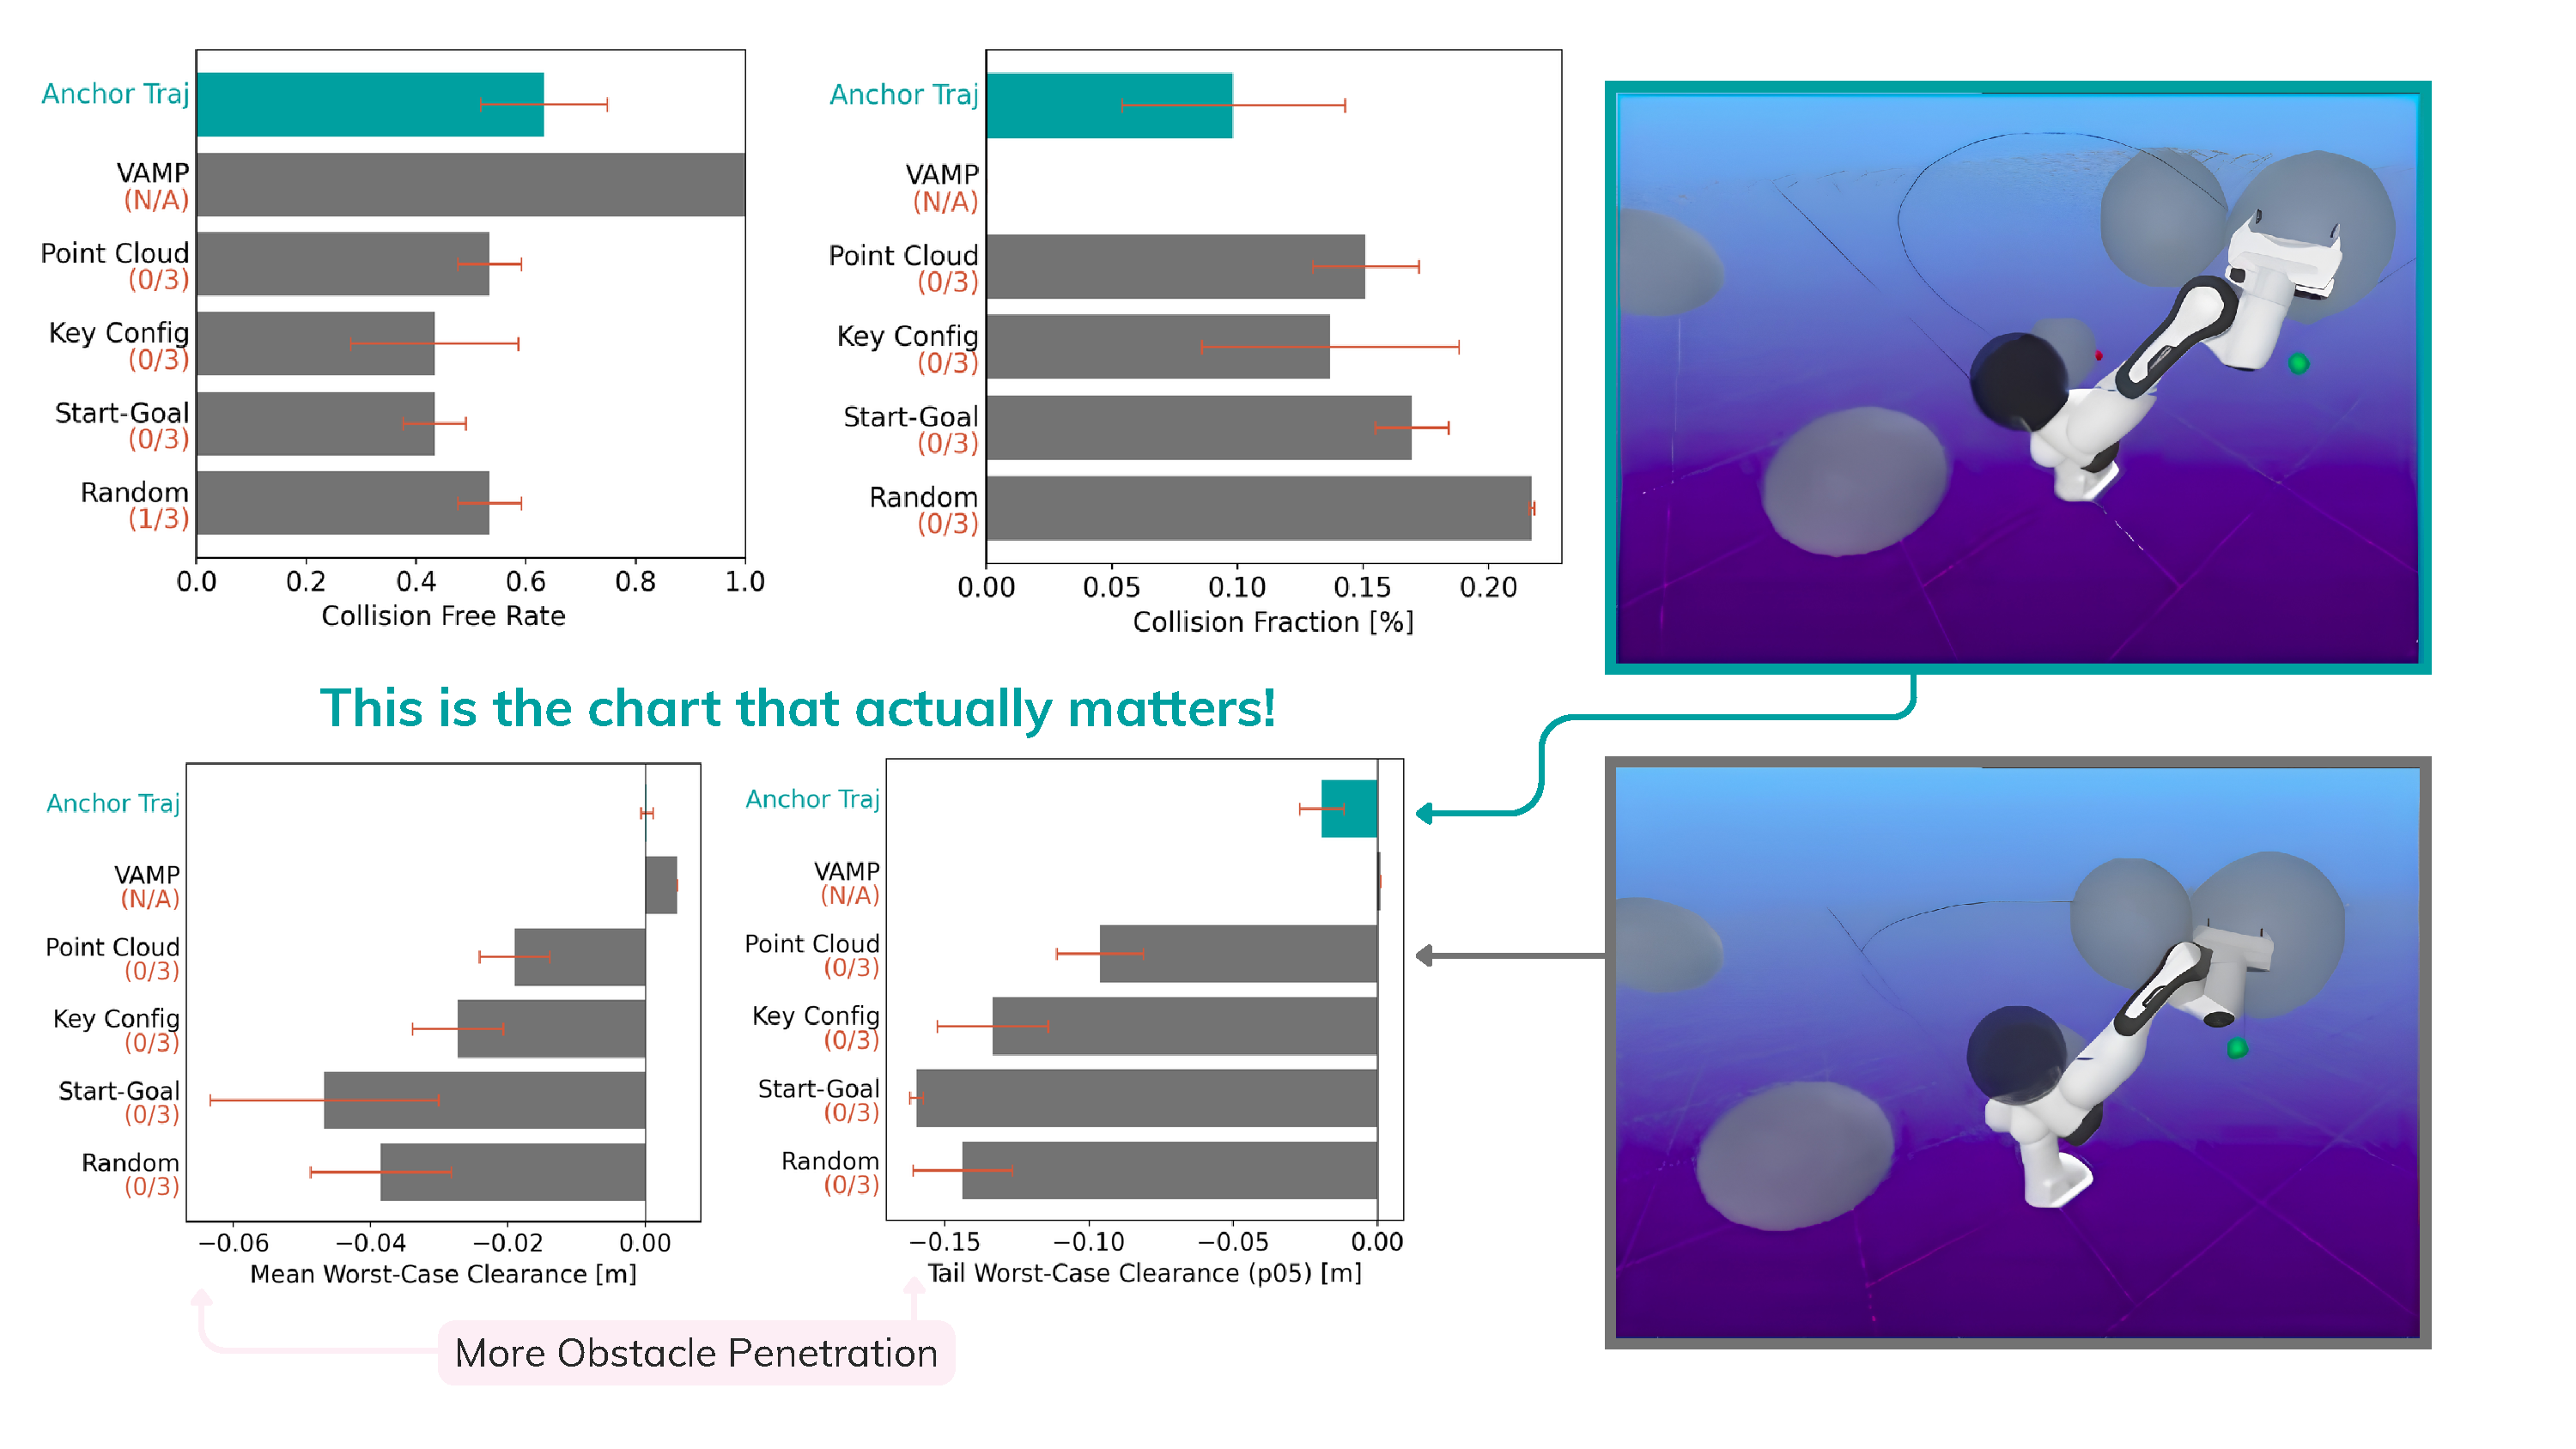
\includegraphics[width=\textwidth]{ThesisFilePkg/figs/charts-anchor.pdf}
  \caption[Collision-avoidance evaluation comparing anchor conditioning to baselines.]{Collision-avoidance evaluation across three training seeds. Anchor Traj denotes the proposed diagnostic anchor conditioning method. VAMP is shown as an oracle-like upper bound rather than a learned conditioning baseline. Point Cloud uses a PointNet++ environment encoder, Key Config uses PRESTO key configurations, Start-Goal does not condition on environment information, and Random uses random environment codes. Anchor Traj provides the strongest overall learned-model performance, with the clearest improvements appearing in collision-severity and worst-case-clearance metrics.}\label{fig:eval}
\end{figure*}

\subsection{Collision-Avoidance Results}

Figure~\ref{fig:eval} summarizes the collision-avoidance results across the learned conditioning methods and the VAMP reference ceiling. The main result is that anchor conditioning improves the quality of generated trajectory initializations. While the collision-free rate provides a useful binary success measure, the clearest advantage of Anchor Traj appears in the violation-severity metrics: collision fraction, collision steps, and worst-case clearance. These metrics are especially important in this setting because the diffusion model is used to generate trajectory candidates that may be passed to a downstream planner or optimizer. A trajectory that is not fully feasible but has fewer and less severe collisions is a better initialization than one that penetrates obstacles deeply or remains in collision for a large portion of the rollout.

\subsubsection{Collision-Free Rate}

Anchor Traj achieves the strongest collision-free rate among the learned diffusion-based conditioning methods. VAMP remains the reference ceiling, as expected, because it represents the performance of the underlying trajectory source rather than a learned conditioning baseline. Among the learned methods, Anchor Traj outperforms Point Cloud, Key Config, Start-Goal, and Random conditioning on average.

The comparison with Start-Goal shows that environment information is necessary: conditioning only on the planning query is insufficient when the same start and goal can require different motions in different environments. The comparison with Point Cloud shows that providing geometric information alone does not guarantee the best planning behavior, since the diffusion model must still learn which geometric distinctions are relevant for feasibility. The comparison with Random is also informative. Random environment codes can sometimes help because they give the model a way to distinguish environments, but they do not encode how each environment constrains motion. Anchor signatures provide a more structured conditioning signal because each bit corresponds to the feasibility response of a diagnostic trajectory probe.

At the same time, the collision-free-rate improvement should not be overstated. The margin over some baselines is moderate, and Random conditioning performs competitively in some seeds. This suggests that binary success rate alone does not fully capture the benefit of the proposed representation. For that reason, the remaining metrics are important for understanding how anchor conditioning changes the quality of the generated trajectories.

\subsubsection{Collision Fraction and Collision Steps}

Collision fraction and collision steps measure the severity of constraint violation rather than only whether a trajectory is completely collision-free. These metrics show a clearer advantage for Anchor Traj. Compared with the other learned conditioning methods, Anchor Traj produces trajectories with a smaller fraction of waypoints in collision and fewer collision steps along the trajectory.

This result is important because diffusion-generated trajectories are often used as initial guesses. A failed trajectory with a small number of colliding waypoints is much closer to feasibility than a failed trajectory that remains in collision for a large part of its duration. In this sense, Anchor Traj improves not only the probability of producing a fully feasible sample, but also the quality of infeasible samples. The generated trajectories are shifted closer to the feasible set, which should reduce the amount of correction required from a downstream optimizer or trajectory-repair procedure.

This supports the central motivation for behavioral anchor conditioning. The anchor signature does not attempt to reconstruct the full scene geometry. Instead, it exposes how the environment responds to representative motion probes. The resulting code appears to provide the denoising model with information that is directly relevant to avoiding constraint violations.

\subsubsection{Worst-Case Clearance}

Worst-case clearance provides another measure of trajectory quality. It evaluates the minimum clearance along a trajectory, making it sensitive to rare but severe obstacle penetrations. Negative clearance values indicate penetration into obstacles, so values closer to zero from below indicate less severe collision when a trajectory is not fully collision-free.

Anchor Traj achieves the best worst-case clearance behavior among the learned conditioning methods. Both the mean worst-case clearance and the lower-tail clearance improve relative to Point Cloud, Key Config, Start-Goal, and Random conditioning. The tail metric is particularly important because it captures severe failure cases. A method that occasionally produces deeply penetrating trajectories may be difficult for a downstream optimizer to repair, even if its average performance appears reasonable.

The clearance results therefore strengthen the conclusion from the collision-fraction metrics. Anchor conditioning does not merely improve binary feasibility. It also reduces the severity of the remaining failures. This is the strongest empirical evidence that the proposed representation provides better trajectory initializations for constrained generation.

\subsection{Discussion of Results}

Overall, the collision-avoidance results support the hypothesis that behaviorally defined environment codes can be more useful for trajectory diffusion than purely perceptual or hand-designed conditioning inputs. Point Cloud conditioning provides direct geometric information, but the model must learn from data which geometric features matter for feasible motion. Key Config conditioning provides a more structured representation, but it may not preserve all distinctions that affect the generated trajectory distribution. Start-Goal conditioning confirms that the planning query alone is insufficient, and Random conditioning shows that simply assigning different identifiers to environments does not consistently capture the structure needed for feasibility.

The main advantage of Anchor Traj is that its conditioning signal is constructed from constraint responses. Each bit in the signature records whether a selected diagnostic trajectory snippet is feasible in the environment. As a result, environments are distinguished when they impose different feasibility outcomes on representative motions. This gives the diffusion model a compact input that is aligned with the downstream planning objective.

The most important interpretation of the results is that Anchor Traj produces better initial guesses. Collision-free rate is useful, but it is a strict binary metric. Collision fraction, collision steps, and worst-case clearance show how close generated trajectories are to feasibility when they fail. On these measures, anchor conditioning provides a clearer improvement. This matters because trajectory diffusion is often used not as a final planner by itself, but as a generator of candidate trajectories that can be refined, optimized, or checked by a downstream planning system.

These results should be interpreted within the scope of the experiment. The empirical evaluation in this chapter validates anchor conditioning for geometric collision avoidance. The formulation is compatible with other binary constraint oracles, but the experiments here do not yet demonstrate improved performance for dynamic, torque, contact, or task-specific constraints.

\section{Discussion}

\subsection{Extension to Other Constraint Oracles}

The anchor-conditioning interface is not specific to collision checking. The only requirement is access to a binary feasibility oracle that evaluates whether a trajectory snippet satisfies the constraints associated with an environment. In the collision-avoidance experiments above, this oracle checks geometric validity. However, the same construction could be applied with a different oracle that incorporates dynamic feasibility, torque limits, contact constraints, visibility constraints, or task-specific rules.

Under this broader view, the semantics of the constraint checker may change, but the representation interface remains the same. A fixed set of anchors is evaluated in each environment, and the resulting binary responses form a signature used to condition the trajectory diffusion model. For example, a geometric oracle would produce a signature indicating which anchor snippets are collision-free, while a dynamics-aware oracle could produce a signature indicating which snippets satisfy both collision and torque constraints.

The experiments in this chapter validate the approach only for geometric collision constraints. Extending the empirical evaluation to richer constraint models remains future work. Nevertheless, the formulation suggests that diagnostic anchor conditioning can be understood as a general method for converting arbitrary feasibility queries into compact behavioral environment codes.


\subsection{Limitations}

The first limitation is that the empirical evaluation in this chapter focuses on geometric collision avoidance. The anchor-conditioning formulation is written in terms of a general binary feasibility oracle, and the same interface could be used for dynamic, torque, contact, visibility, or task-specific constraints. However, the results presented here only validate the method for collision constraints. Demonstrating the same benefits for richer constraint models remains future work.

Second, the method assumes access to a constraint oracle that can evaluate anchor snippets in each environment. In the collision-avoidance setting, this oracle is a collision checker. In other settings, the oracle may require dynamics simulation, torque computation, contact reasoning, or task-level feasibility checks. The usefulness of the method therefore depends on whether these feasibility queries are cheaper or easier than solving the full planning problem.

Third, the binary signature discards information about the reason and severity of failure. A snippet that barely violates a clearance threshold and a snippet that deeply penetrates an obstacle both receive the same infeasible label. This binary abstraction is useful because it provides a simple and constraint-agnostic interface, but it may lose information that could help the diffusion model distinguish mild violations from severe ones. Future versions of the method could use multi-valued or continuous anchor responses, such as clearance, penetration depth, torque margin, or constraint residuals.

Fourth, the representation is limited by the selected anchor set. Two environments with identical anchor signatures are treated as equivalent by the downstream diffusion model, even if they differ in ways that are not tested by the selected probes. Increasing the number of anchors can reduce this ambiguity, but it also increases the dimensionality of the conditioning code and the cost of encoding new environments. The quality of the representation therefore depends on whether the candidate snippet library contains probes that expose the constraint variations relevant to the test environments.

Fifth, the current evaluation uses a small number of training seeds. The reported trends suggest that anchor conditioning improves trajectory quality, especially in terms of collision severity and clearance, but additional runs would provide a stronger estimate of variability. More extensive ablations over the number of anchors, the snippet horizon, the candidate snippet source, and random anchor selection would further clarify which parts of the method are most important.

Finally, the chapter argues that better collision fraction and clearance should make generated trajectories better initializations for downstream optimization. This interpretation is supported by the fact that Anchor Traj produces trajectories closer to feasibility, but a complete evaluation should directly measure downstream planner performance, including optimization iterations, repair success rate, and total planning time.

\section{Conclusion}\label{sec:anchor-conclusion}

This chapter presented behavioral anchor conditioning for environment-conditioned trajectory diffusion. The central idea is to represent an environment not by its raw perceptual or geometric description, but by its binary responses to a selected set of diagnostic trajectory snippets. These responses form a compact feasibility signature that approximates behavioral equivalence: environments are distinguished when they permit or forbid different representative motions.

In collision-avoidance experiments, anchor conditioning produced stronger learned-model performance than point-cloud, key-configuration, start-goal-only, and random conditioning baselines. The clearest benefit was not only an improvement in collision-free rate, but a reduction in the severity of failed samples. Anchor-conditioned trajectories had lower collision fraction and improved worst-case clearance, indicating that they are closer to feasibility and therefore better suited as initial guesses for downstream planning or trajectory optimization.

The formulation is more general than the collision checker used in this evaluation. Any constraint model that can produce binary feasibility responses for trajectory snippets can, in principle, be used to construct anchor signatures. However, the empirical validation in this chapter is limited to geometric collision avoidance. Extending the evaluation to dynamic, torque, contact, and task-specific constraints remains an important direction for future work.

Across \cref{ch:payload} and this chapter, amortization reaches its most aggressive form in this thesis: dynamic and geometric feasibility is absorbed into the parameters of a learned generative model and recovered at sampling time, rather than recomputed online or stored as an explicit structure.
Where payload conditioning targeted a specific dynamic capability, behavioral anchor conditioning targets feasibility itself, providing a task-agnostic interface between learned generation and classical optimization.
\cref{ch:discussion} steps back to draw the broader lessons that connect online evaluation, amortized reusable structure, and learned conditional generation into a single account of where knowledge of dynamic feasibility should reside in a manipulation system.
